\documentclass[9pt,final,a4paper]{IEEEtran}

\usepackage{amsmath}
\usepackage{graphicx}
\usepackage{setspace}
\usepackage{cite}
\usepackage{subfig}
\graphicspath{ {./images/} }
\usepackage{caption}
\usepackage{kotex}
\usepackage{hyperref}
\usepackage{inputenc}
\usepackage{csquotes}
\usepackage{float}

\singlespacing

\begin{document}

\title{\LARGE Improving Automatic Speech Recognition Model Peformance on Korean Dysarthric Speech with Transfer Learning}

\author{Sanghyeon Kim (Sogang University)\\ \href{mailto:anton3017@sogang.ac.kr}{anton3017@sogang.ac.kr}}

\maketitle

\begin{abstract}
    Dysarthric speech recognition has been a challenge for many commercially available ASR systems.
    In general, state-of-the-art automatic speech recognition (ASR) systems perform as good as or even better than humans on normal speech, but lack performance in dysarthric speech.
    One of the major causes of this discrepancy has been the lack of dysarthric speech data available to train any ASR model compared to normal speech data.
    With publicly available large Korean dysarthric speech dataset, this project aims to improve performance of Korean dysarthric ASR model using pre-trained base model.
\end{abstract}

\section{Introduction}

\subsection{Dysarthric Speech Characteristic}

\captionsetup{justification=centering}
\begin{figure}[h]
    \caption{\small Wavelength and Spectrogram Representation of Normal Speech and Dysarthric Speech}
    \subfloat[Dysarthric Speech]{
        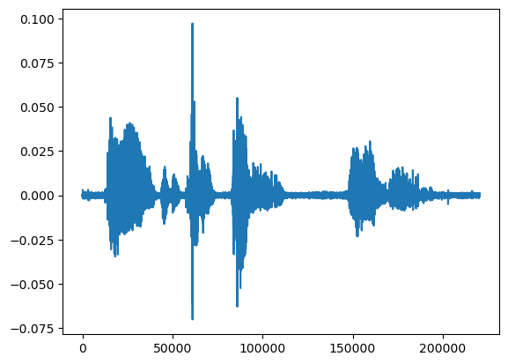
\includegraphics[width=0.47\columnwidth]{Picture1.png}
    }
    \subfloat[Normal Speech]{
        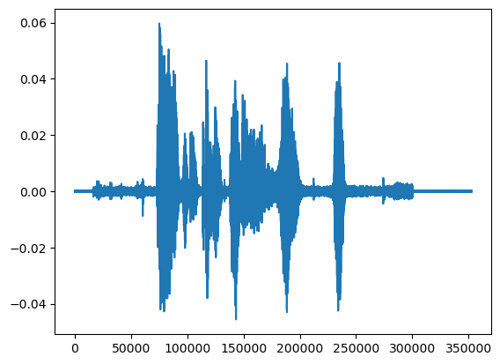
\includegraphics[width=0.47\columnwidth]{Picture2.png}
    }
    \\
    \subfloat[Dysarthric Speech]{
        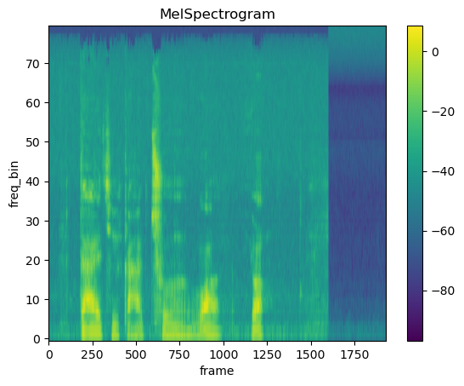
\includegraphics[width=0.47\columnwidth]{Picture3.png}
    }
    \subfloat[Normal Speech]{
        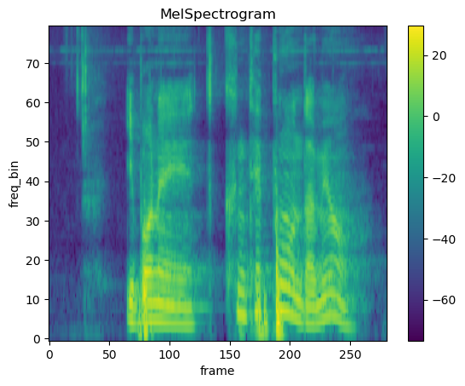
\includegraphics[width=0.47\columnwidth]{Picture4.png}
    }
\end{figure}

The above figures show short speech of two different speakers. Dysarthric speaker has cranial nerve disorder, and the other speaker does not have any disorder.
Dysarthric speaker spoke \enquote{Is the weather cold?} in Korean, and normal speaker spoke \enquote{Have you heard that a large typhoon is coming?}.
There are some noticeable differences between the two speeches. First, dysarthric speech has longer pauses in between utterances than that of normal speech.
Moreover, by comparing the MelSpectrogram of two speeches, the dysarthric speaker is found to have weaker vocalization strength compared to normal speaker.
Hence, dysarthric speaker's utterance is more susceptible to background noise, which decreases the accuracy of speech recognition.
Also, due to longer pauses in between utterances in dysarthric speech, ASR systems trained on normal speech do not properly model this trait\cite{cite2}.

\subsection{Datasets Description}

Datasets are downloaded from \href{https://aihub.or.kr/aihubdata/data/view.do?currMenu=115&topMenu=100&aihubDataSe=realm&dataSetSn=123}{Normal Speech Dataset Link}, \href{https://aihub.or.kr/aihubdata/data/view.do?currMenu=115&topMenu=100&aihubDataSe=realm&dataSetSn=608}{Dysarthric Speech Dataset Link}.
These datasets can also be searched at \href{https://aihub.or.kr/}{AI Hub}.

\subsubsection{Normal Speech Data}

ETRI conversational speech data with 1000 recording hours of 2000 male and female speakers.
Audio format is 16bits headerless linear PCM with sampling rate of 16KHz.

\begin{table}[h]
    \caption*{Training Dataset}
    \vspace*{-3mm}
    \begin{center}
        \begin{tabular}{|c|c|c|}
            \hline
            Category & Male & Female \\ [0.5ex] 
            \hline\hline
            Number of Speakers & 923 (46\%) & 1,077(54\%) \\ 
            \hline
            Total & \multicolumn{2}{|c|}{2000} \\
            \hline
        \end{tabular}
    \end{center}
\end{table}

Evaluation datasets are separated into two categories.

\begin{table}[h]
    \begin{center}
        \begin{tabular}{|c|c|}
            \hline
            Category & Recorded Hours \\ [0.5ex] 
            \hline\hline
            Validation Set & 2.6 \\ 
            \hline
            Test Set & 3.8 \\
            \hline
        \end{tabular}
    \end{center}
\end{table}

\subsubsection{Dysarthric Speech Data}

About 150 recording hours of training dataset. Unlike normal speech dataset, audio format is \emph{.wav} recorded at 44.1KHz sampling rate.
Self implemented data module in PyTorch down samples this audio to 16KHz, so that the MelSpectrogram window matches for both normal and dysarthric speech.

\begin{table}[h]
    \caption*{Training Dataset}
    \vspace*{-3mm}
    \begin{center}
        \begin{tabular}{|c|c|c|}
            \hline
            Category & Male & Female \\ [0.5ex] 
            \hline\hline
            Number of Speakers & 142 (41\%) & 201 (59\%) \\ 
            \hline
            Total & \multicolumn{2}{|c|}{343} \\
            \hline
        \end{tabular}
    \end{center}
\end{table}
About 217 recording hours of evaluation dataset.
\begin{table}[h]
    \caption*{Evaluation Dataset}
    \vspace*{-3mm}
    \begin{center}
        \begin{tabular}{|c|c|c|}
            \hline
            Category & Male & Female \\ [0.5ex] 
            \hline\hline
            Number of Speakers & 490 (51\%) & 469(49\%) \\ 
            \hline
            Total & \multicolumn{2}{|c|}{959} \\
            \hline
        \end{tabular}
    \end{center}
\end{table}
\vspace*{-5mm}

Evaluation dataset is too large. Hence, only the first 7 hours (approx.) of recordings are used as validation and test data.
7 hour recordings are separated evenly into validation and test data.
For dysarthric speech data, only cranial nerve disorder patient data have been used for training and evaluation.
In fact, there is only cranial nerve disorder evaluation data available.
Moreover, for dysarthric speech dataset, recordings with transcripts that exceed 1000 tokens after tokenization are excluded because of GPU memory overload during training.

\subsection{Model Type}

Model used in this project is Conformer RNN-T. Conformer is used as encoder and RNN-T is used as decoder in this ASR system.

\subsection{Training Steps}

\subsubsection{Text Normalization}

Normal speech data provided by ETRI require parts of transcriptions to be transcribed into either \emph{phonetic transcription} or \emph{orthographic transcription}.
Also, there are several special keys for certain acoustic characteristics such as occurances of noise, unclear words, etc.

\subsubsection{Tokenizer Training}

SentencePiece model is trained with normalized transcript data. Model is trained with Unigram tokenization.
Normalized transcript from normal speech data is used to train this model.

\subsubsection{Global Stats}

Audio needs to be normalized before training. Since calculating average and standard deviations needed for nomalization of each batch require additional computation during training, it is better to calculate these values before training begins.
Statistics for both normal speech and dysarthric speech are saved on separate json files.

\subsubsection{Distributed Data Parallel}

Distributed Data Parallel is a module in PyTorch that allows you to train a neural network on multiple GPUs or machines.
DDP works by splitting the input data into batches and distributing them across the devices\cite{cite4}.

\subsubsection{Base Model Training}

Base model is trained on normal speech dataset. Two different Conformer RNN-T models are trained.
One with large parameter size, and the other with smaller parameter size.

\subsubsection{Transfer Learning}

Dysarthric ASR model is trained with pre-trained based model in the previous step. Dropout rate and learning rates per layer are adjusted for transfer learning\cite{cite6}\cite{cite7}.

\section{Dataset Preprocessing and Tokenizer Training}

Normal speech dataset had to be preprocessed to clean up special tag characters as well as transcription decision making.
Dysarthric speech dataset contains minimal special tag characters.
Special tag characters used in speech datasets includes the following.

\begin{center}
    \begin{table}[h]
        \caption*{}
        \vspace*{-3mm}
        \begin{center}
            \begin{tabular}{|c|c|}
                \hline
                Category & Notation \\ [0.5ex] 
                \hline\hline
                Meta Symbol & \textquote*{/}, \textquote*{(}, \textquote*{)}, \textquote*{[}, \textquote*{]}, \textquote*{*}, \textquote*{+} \\ 
                \hline
                Noise & \textquote*{lg/}, \textquote*{br/}, \textquote*{n/} \\
                \hline
                Meaningless Words & \textquote*{*/} (* is fill-in for character(s))\\
                \hline
                Transcription & \textquote*{(\emph{phonetic})/(\emph{orthographic})}\\
                \hline
                Special Tags & \textquote*{b/}, \textquote*{l/}, \textquote*{o/}, \textquote*{n/}, \textquote*{u/} \\
                \hline
            \end{tabular}
        \end{center}
    \end{table}
\end{center}

Unlike normal speech data provided by ETRI, dysarthric speech does not provide options for phonetic or orthographic notations.
Hence, numbers are typed orthographically rather than phonetically in this dataset.
To prevent Out-Of-Vocabulary (OOV) in tokenization of dysarthric speech transcript, tokenizer being trained must learn both representation of numbers.
Therefore, for any occurances of numeric text in normal speech dataset, orthographic or phonetic transcript is randomly chosen during text normalization.
Tokenizer vocabulary size is set to 10000.

\section{Model Architecture: Conformer RNN-Transducer}

\subsection{Conformer}

\begin{figure}[ht]
    \centering
    \subfloat[Conformer]{
        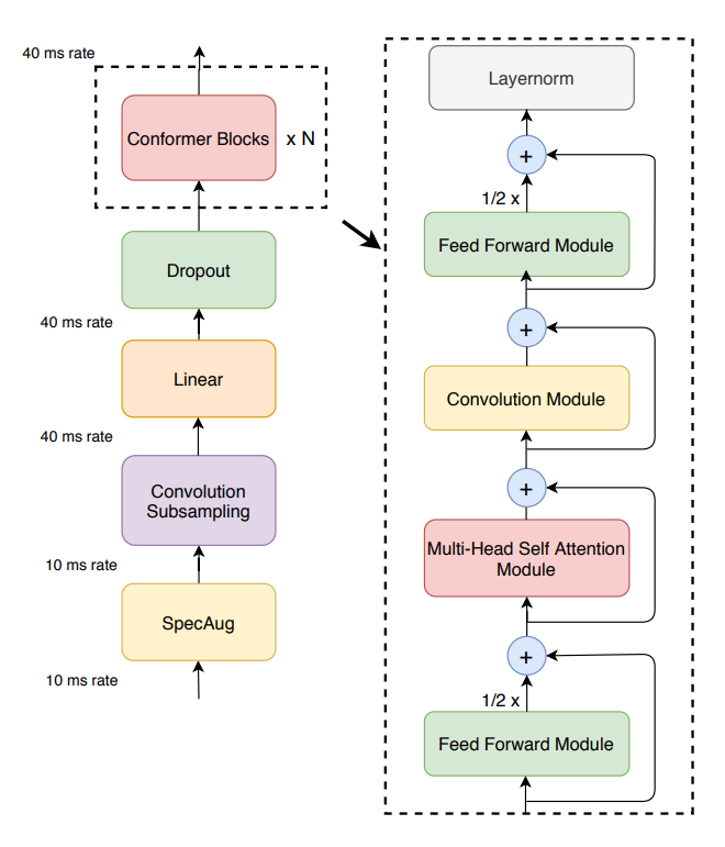
\includegraphics[width=0.5\columnwidth]{Picture5.png}
    }
\end{figure}

Encoder part of this project's ASR system uses a Conformer model.
Conformer model is a type of neural network architecture that combine convolutional, recurrent, and self-attention layers to achieve state-of-the-art results in speech recognition tasks.
They are based on the idea that convolutional layers can capture local dependencies, while recurrent, self-attention layers can capture long-term dependencies, and global context.
Conformer model consist of four main components: a convolutional module, a multi-head self-attention module, a feed-forward module, and a recurrent module.
The convolutional module applies a 1D depthwise separable convolution to the input, which reduces the number of parameters and improves the efficiency of the model.
The multi-head self-attention module computes the attention weights between each pair of input elements, which allows the model to learn the semantic relationships and dependencies between them.
The feed-forward module applies two linear transformations with a non-linear activation function in between, which adds non-linearity and expressiveness to the model\cite{cite5}.

The recurrent module applies LSTM or any other RNN-like module to the input, which enables the model to capture the temporal dynamics and sequential information.
By stacking these modules as encoder-decoder(or predictor) structure, conformer models can encode the input sequence into a high-level representation and decode it into an output sequence, such as a transcription or a translation\cite{cite5}.

\subsection{RNN-Transducer}

\begin{figure}[H]
    \centering
    \subfloat[RNN-Transducer]{
        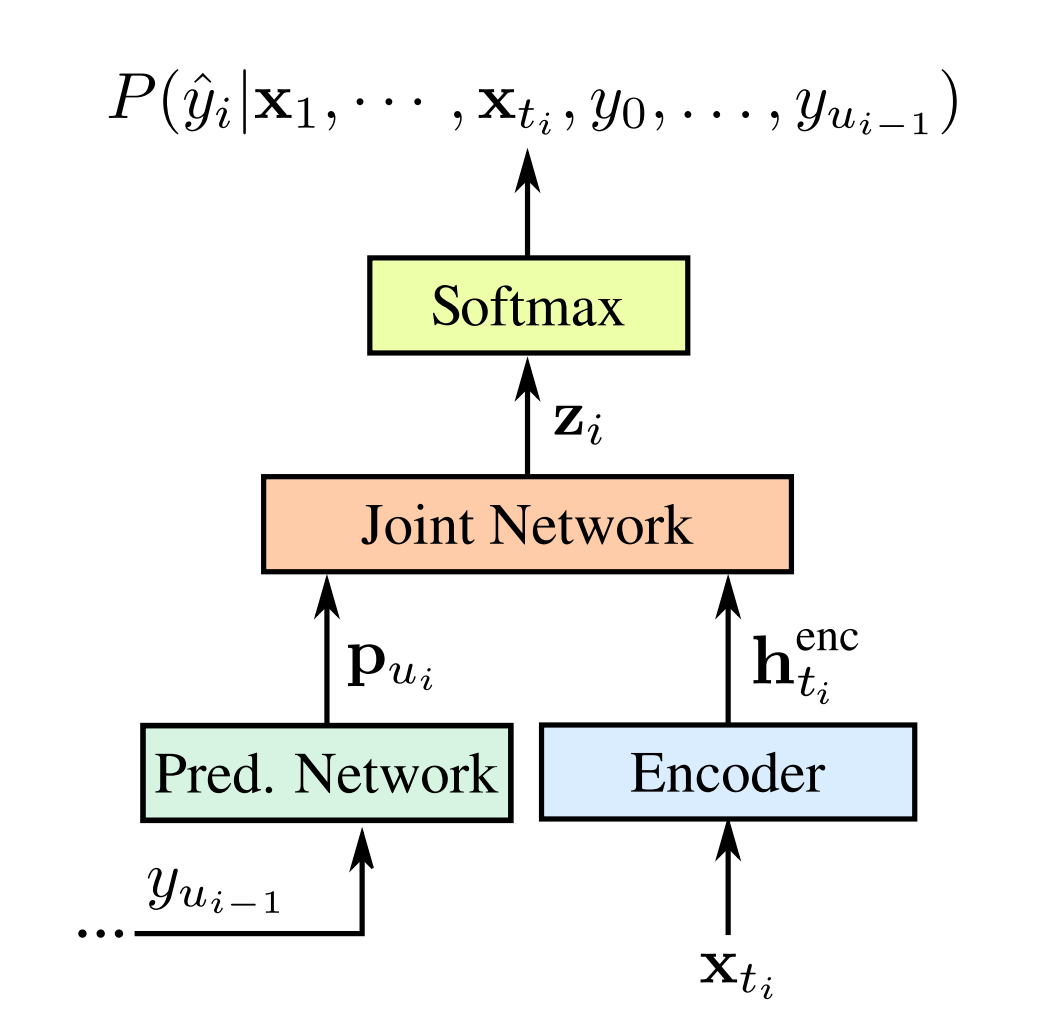
\includegraphics[width=0.5\columnwidth]{Picture6.png}
    }
\end{figure}

RNN-T (Recurrent Neural Network Transducer) is a neural network architecture for ASR that combines the acoustic model, language model, punctuation model, and inverse text normalization into one single model\cite{cite3}.
RNN-T consists of three components: an encoder, a predictor, and a joint network.
The encoder processes the input audio features and produces a high-level representation.
The predictor predicts the next output symbol based on the previous output symbols.

The joint network combines the encoder and predictor outputs and computes the probability distribution over the output symbols.
RNN-T can handle variable-length input and output sequences without requiring any alignment information\cite{cite3}.
RNN-T can also control the latency during inference by adjusting the number of encoder steps before invoking the predictor and joint network.
RNN-T has been shown to achieve comparable or even better accuracy and efficiency than traditional hybrid ASR systems like RNN-HMM on various datasets.

\subsection{Large Conformer RNN-T Model}

\begin{table}[H]
    \caption*{Model Parameters}
    \vspace*{-3mm}
    \begin{center}
        \begin{tabular}{|c|c|}
            \hline
            Parameter Type & Value \\ [0.5ex] 
            \hline\hline
            Input Dimension & 80 \\
            \hline
            Encoding Dimension & 1024 \\
            \hline
            Conformer Input Dimension & 256 \\
            \hline
            Number of Heads & 4 \\
            \hline
            Conformer Dropout & 0.2 \\
            \hline
            Symbol Embedding Dimension & 256 \\
            \hline
            Number of LSTM Layers & 4 \\
            \hline
            LSTM Hidden Dimension & 512 \\
            \hline
            LSTM Dropout & 0.2 \\
            \hline
        \end{tabular}
    \end{center}
\end{table}

This model contains approximately 44.1M parameters.

\subsection{Small Conformer RNN-T Model}

\begin{table}[H]
    \caption*{Model Parameters}
    \vspace*{-3mm}
    \begin{center}
        \begin{tabular}{|c|c|}
            \hline
            Parameter Type & Value \\ [0.5ex] 
            \hline\hline
            Input Dimension & 80 \\
            \hline
            Encoding Dimension & 256 \\
            \hline
            Conformer Input Dimension & 128 \\
            \hline
            Number of Heads & 2 \\
            \hline
            Conformer Dropout & 0.2 \\
            \hline
            Symbol Embedding Dimension & 128 \\
            \hline
            Number of LSTM Layers & 3 \\
            \hline
            LSTM Hidden Dimension & 128 \\
            \hline
            LSTM Dropout & 0.2 \\
            \hline
        \end{tabular}
    \end{center}
\end{table}

This model contains approximately 11M parameters.

\section{Model Training}

Both base model training and dysarthric speech transfer learning steps were done on \href{https://jarvislabs.ai/}{JarvisLab}'s GPU instance with two A6000 GPUs.
Training time took approximately 48 hours for the base model, and 16 hours for the transfer learning step.
Training time was significantly reduced by passing multi-gpu model to DDP.
In the transfer learning step, dropout rate was increased to 0.6 and first half layers of conformer and first half of LSTM layers were frozen by giving 0 learning rate on those layers.

\section{Results}
\vspace*{-2ex}
\begin{table}[ht]
    \caption*{Character Error Rate(CER) of Base Model}
    \vspace*{-3mm}
    \begin{center}
        \begin{tabular}{|c|c|c|}
            \hline
            Model Type & Normal Speech & Dysarthric Speech \\ [0.5ex] 
            \hline\hline
            Large & 12.1\% & 33.7\% \\ 
            \hline
            Small & 18.3\% & 38.4\% \\
            \hline
        \end{tabular}
    \end{center}
\end{table}

It can be seen that the model with more parameters perform better than the model with less parameters in both speech datasets.
The performance difference between the two models in normal speech and dysarthric speech is approximately the same.
However, when comparing CER of each model between normal speech and dysarthric speech in more detail, it can be said that the small model has less performance gap compared to large model ($\Delta$20.1\% compared to $\Delta$21.6\%).
This could result from the fact that model with less parameter is a more generalized model than the larger model, of which the larger model could have fitted more to normal speech.

\begin{table}[ht]
    \caption*{Character Error Rate(CER) after Transfer Learning}
    \vspace*{-3mm}
    \begin{center}
        \begin{tabular}{|c|c|c|}
            \hline
            Model Type & Normal Speech & Dysarthric Speech \\ [0.5ex] 
            \hline\hline
            Large & 17.6\% & 20.3\% \\ 
            \hline
            Small & 23.7\% & 29.1\% \\
            \hline
        \end{tabular}
    \end{center}
\end{table}

After transfer learning step is complete. Both models gain CER in normal speech, which means it lost performance in recognizing regular speech.
Both models reduced CER of dysarthric speech, but larger model managed to gain more performance than smaller model.
In dysarthric speech, large model reduced CER by $\Delta$13.4\% and smaller model reduced CER by $\Delta$9.3\%.
However, both models gained CER (losing performance) after transfer learning step.
The smaller model appears to have lost more performance than the larger model.
This could result from the fact that smaller model has less parameter to model acoustic characteristics of both normal speech and dysarthric speech.


\section{Application}

Well optimized RNN-T systems can be run on mobile devices.
Benefits of running this system comes from the fact that RNN-T models have minimal latency between input and output, which helps to run ASR systems real-time.
With optimization methods such as state caching techniques used in other RNN language models, inference is much faster and compution becomes more efficient\cite{cite1}.
Mobile application that utilizes an improved Conformer RNN-T system with contextual biasing is currently in development.

\begin{figure}[H]
    \centering
    \subfloat[Android Studio]{
        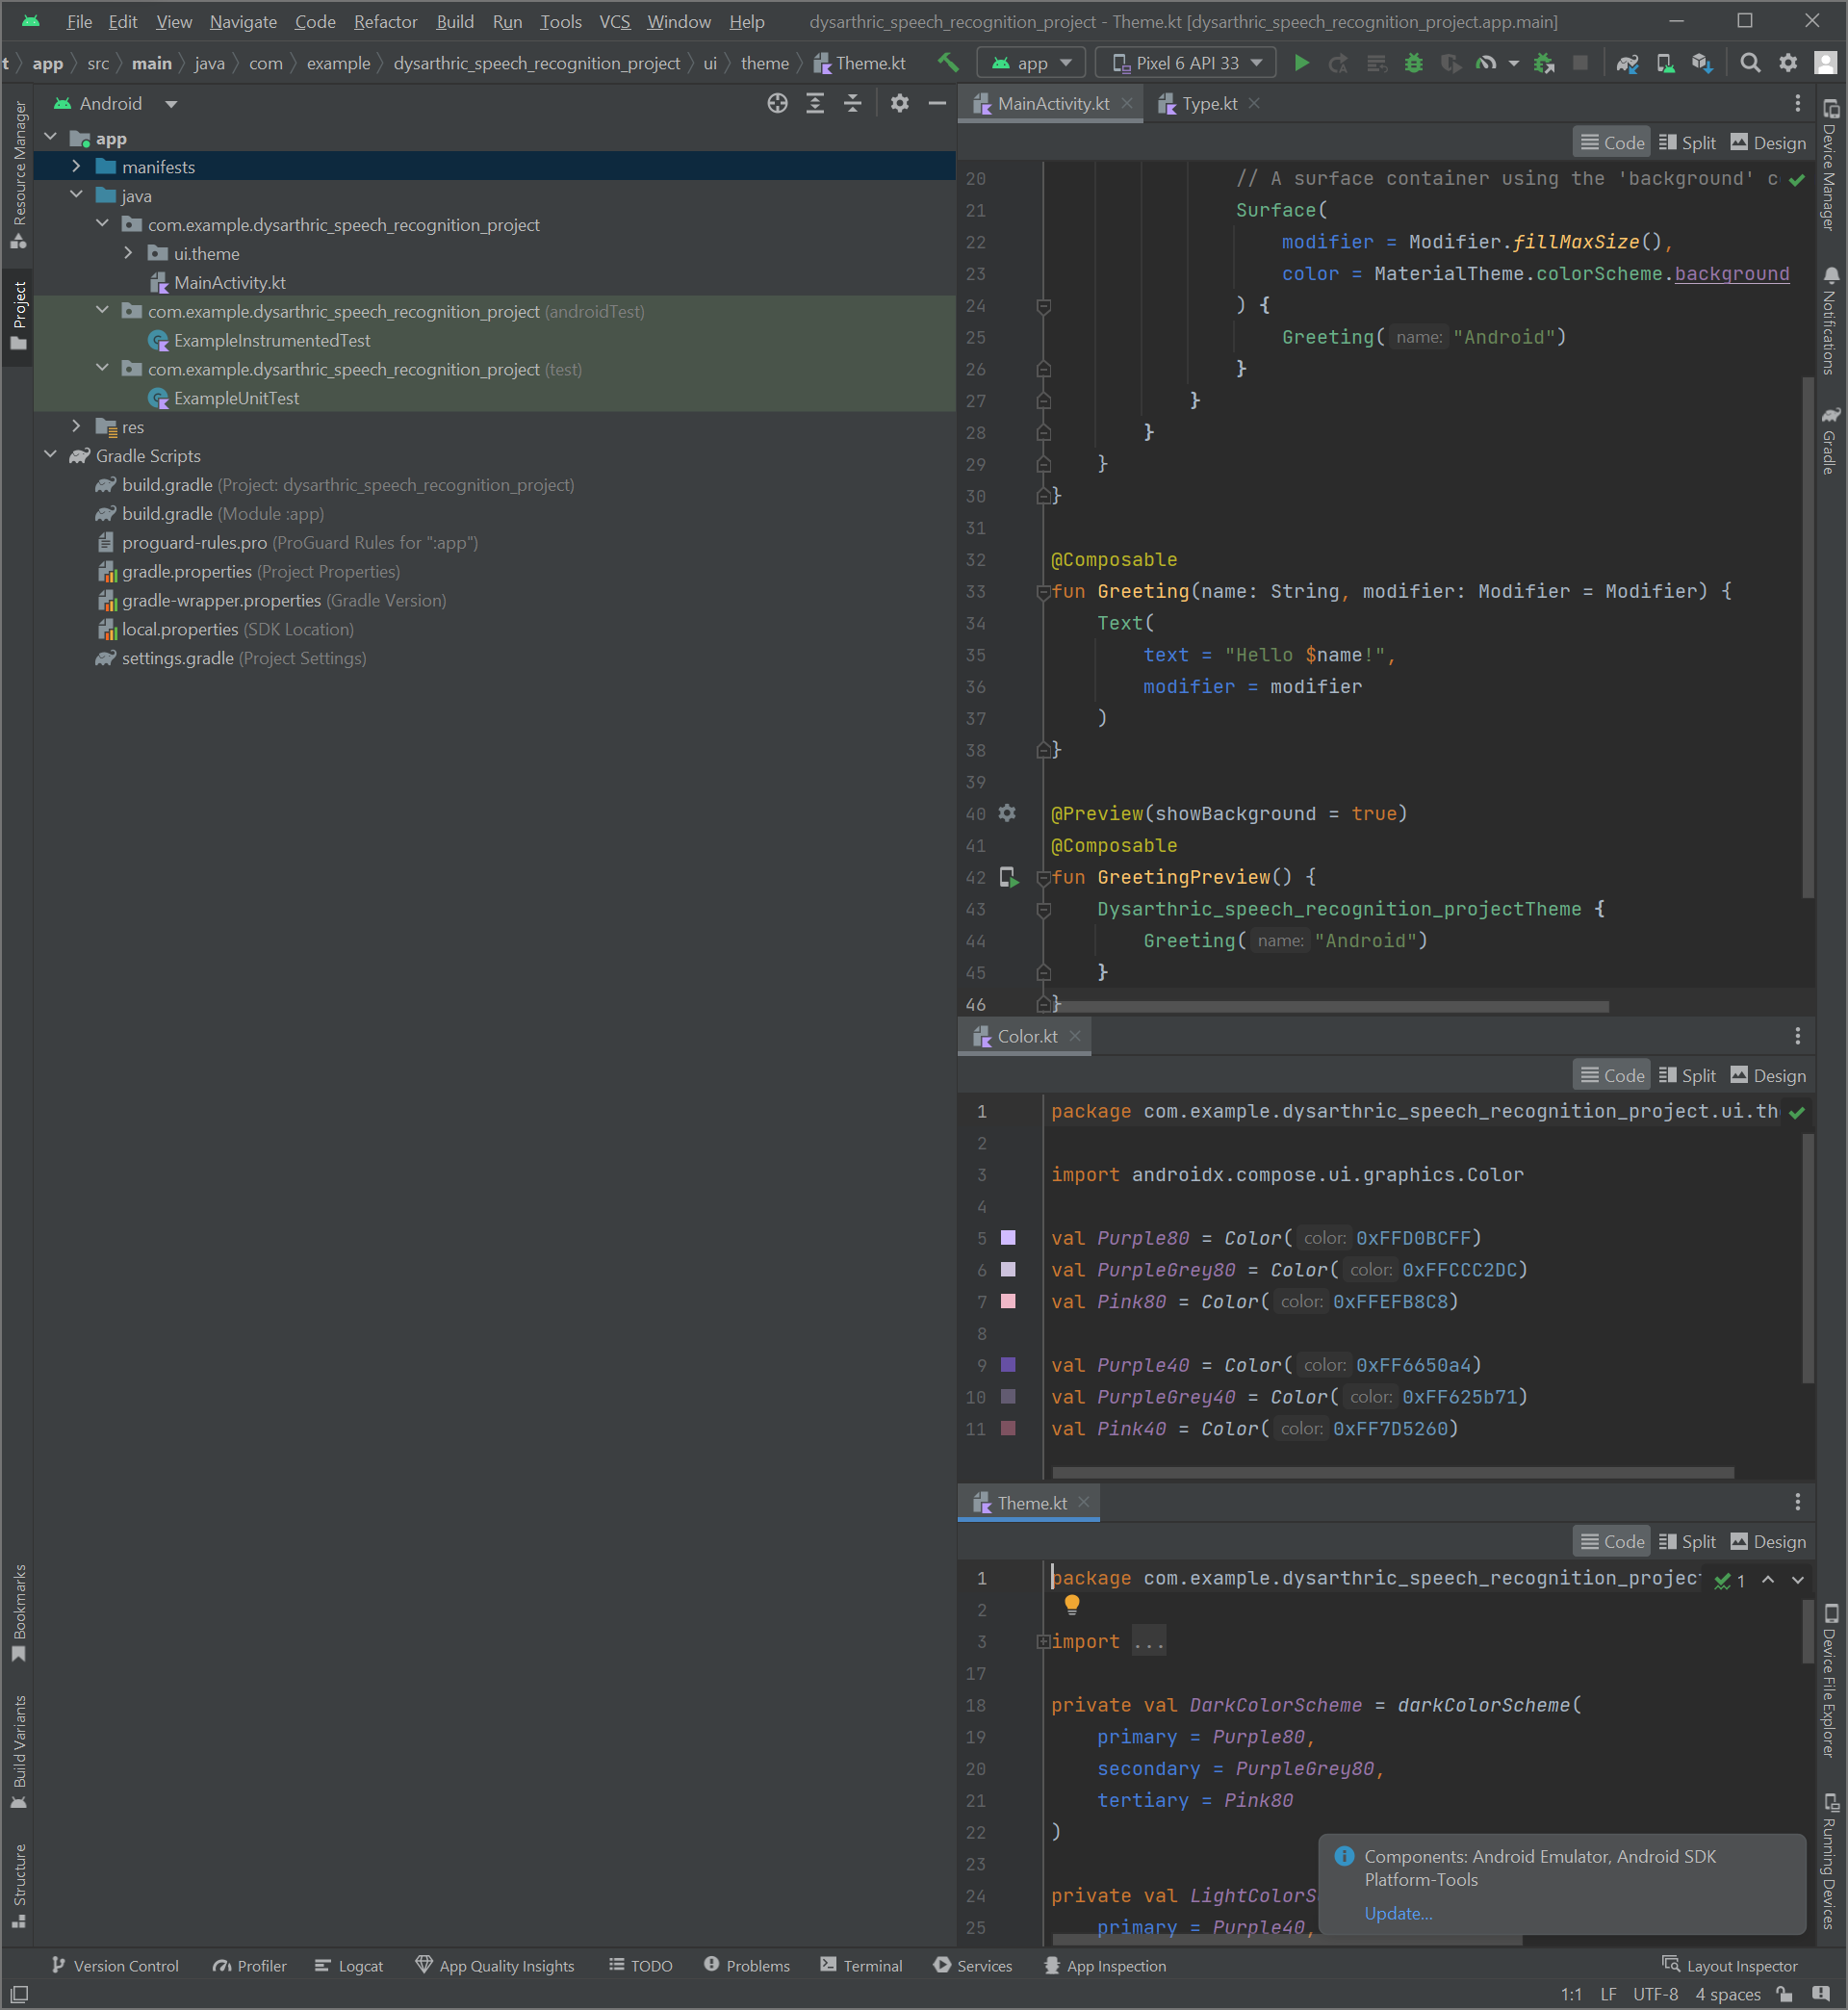
\includegraphics[width=0.4\columnwidth]{Picture7.png}
    }
\end{figure}

\section{Conclusion}

In this research, E2E (End-to-End) ASR system based on Conformer RNN-T was used to train Korean dysarthric speech recognition model. 
The goal was to find if transfer learning method would improve dysarthric speech recognition performance of a model pre-trained on normal speech.
With limited computation resources or data, transfer learning can improve model performance despite these limited resources.
This research showed that with relatively small dysarthric speech training data compared to normal speech, the model pre-trained on normal speech has reduced CER on dysarthric speech after additional training.
If this model is to be trained on dysarthric speech dataset that is not limited to certain disorder, it could have better recognition accuracy on a general group of dysarthric speakers.
Moreover, by taking advantage of real-time processing power of RNN-T model, a useful mobile application could be implemented to help communication between normal speakers and dysarthric speakers.

\bibliography{ref.bib}
\bibliographystyle{plain}
\end{document}